\documentclass[12pt,twocolumn]{article}
\usepackage[margin=1.5cm]{geometry}
\usepackage{amsmath}
\usepackage{graphicx}
\usepackage{hyperref}
\title{Faraday's Law and Mutual Inductance}
\author{Prof. Jordan C. Hanson}

\begin{document}
\small
\maketitle

\section{Introduction}

\begin{figure}[ht]
\centering
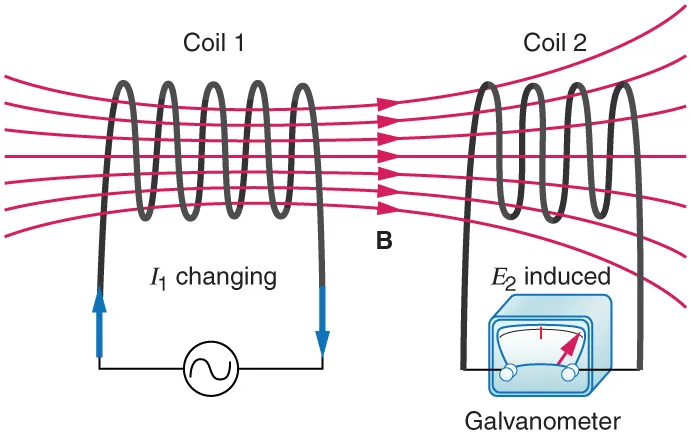
\includegraphics[width=0.45\textwidth]{mutual.png}
\caption{\label{fig:mutual} \textit{Mutual inductance} exists in transformers and other systems with pairs of solenoids or coils.}
\end{figure}

\noindent
In this lab, we will explore the relationship between an oscillating B-field created by one coil, and the induced emf in another coil.  We will refer to the former as the transmitting coil, TX, and the latter as the receiving coil, RX.  Let $\mathcal{E}$ represent the induced emf in the RX coil, $M$ be the mutual inductance, and $I_{\rm TX}$ be the current in the TX coil.  Faraday's Law may be written in the following form:
\begin{equation}
\mathcal{E}_{\rm RX} = - M \frac{\Delta I_{\rm TX}}{\Delta t}
\end{equation}
By symmetry, we can show that
\begin{equation}
\mathcal{E}_{\rm TX} = - M \frac{\Delta I_{\rm RX}}{\Delta t}
\end{equation}
That is, if we reverse the roles of our TX and RX coils, the constant of proportionality between induced $\mathcal{E}$ and changing current will be the same.

\section{Mathematics}

To interpret the main results of this lab activity, we need to show that $\mathcal{E}_{\rm RX}$ is proportional to the frequency of $I_{\rm TX}$.  Start with Faraday's Law in the form with inductance,
\begin{equation}
\mathcal{E}_{\rm RX} = - L\frac{\Delta I_{\rm TX}}{\Delta t}
\end{equation}
Let us consider the case as $\Delta t \to 0$.  This implies that $\Delta I/\Delta t \to dI/dt$, the time-derivative of the current.  The derivative is the slope of a function at a single point.
\begin{equation}
\mathcal{E}_{\rm RX} = - L\frac{dI_{\rm TX}}{dt}
\end{equation}
To evaluate this derivative of current, we need to know how $I_{\rm TX}$ depends on time.  Let's assume we will connect a sine wave to our TX coil, and the coil has some resistance $R$.  Ohm's law gives
\begin{align}
V_{\rm TX}(t) &= I_{\rm TX}R \\
V_0 \sin(\omega t) &= I_{\rm TX}(t) R \\
I_{\rm TX} (t) &= \frac{V_0}{R}\sin(\omega t)
\end{align}
We can always look up the derivative of trigonometric functions in tables\footnote{For this one, see \url{https://en.wikipedia.org/wiki/Differentiation_of_trigonometric_functions}.}:
\begin{align}
f(t) &= A\sin(\omega t) \\
\frac{df}{dt} &= A\omega \cos(\omega t)
\end{align}
Applying this fact to the TX coil current, we find
\begin{equation}
\frac{dI_{\rm TX}}{dt} = \frac{V_0}{R}\omega \cos(\omega t)
\end{equation}
Substituting the real frequency for the angular frequency, we find
\begin{equation}
\frac{dI_{\rm TX}}{dt} = \frac{2\pi V_0}{R} f\cos(2\pi f t)
\end{equation}
Inserting this result into the original equation for Faraday's Law, we find
\begin{equation}
\mathcal{E}_{\rm RX}(t) = -\frac{2\pi V_0 L}{R} f\cos(2\pi f t)
\end{equation}
Two empirical observations should therefore be made:
\begin{enumerate}
\item The frequency of $\mathcal{E}_{\rm RX}(t)$ should be $f$
\item The amplitude of $\mathcal{E_{\rm RX}}(t)$ should be $\propto f$
\end{enumerate}

\section{Experimental Setup}

\noindent
Check that you have the following items at your table:
\begin{itemize}
\item The Analog Arts USB-powered oscilloscope and signal generator unit
\item Two BNC to alligator coaxial cables
\item Two coils of wire, the TX coil and RX coil
\item A 6-foot USB cable to connect the Analog Arts unit to the desktop PC
\item The Analog Arts application icon on the PC desktop window
\item A BNC to BNC coaxial cable.
\end{itemize}

Click on the Analog Arts icon on the PC desktop window.  After a calibration stage, the application should launch.  From the list of functions, choose the oscilloscope.  Explore the Volts/division and microseconds/division controls.  These control the level of zoom on our observed signals.  The oscilloscope \textit{trigger} is represented by an arrow on the left axis.  The trigger allows the scope to draw the received signal if the trigger voltage is exceeded.  The trigger menu allows some customization.  The trigger can activate on a \textit{rising edge}, or a \textit{falling edge.}  When the signal is less than the trigger threshold voltage and then exceeds it, the rising edge option will activate.  When the signal is greater than the threshold but falls below it, the falling edge option will activate.  Normal mode means we are in control of the threshold, and no signal will be drawn unless our trigger is satisfied.  When Auto mode is enabled, signals will be drawn, but not synchronously unless they satisfy the trigger.

Connect the BNC to BNC coaxial cable from the signal generator output to the channel 1 input on the Analog Arts unit.  Now click on the arbitrary wave generator option in the Analog Arts application.  The signal generator window has options for creating custom waveforms, but we will use a sine wave.  Near the bottom of the window, there is a menu for selecting wave type.  Click on sine, and choose a frequency of 1 kHz.  Choose an amplitude VPP (voltage peak-to-peak) of 5000 mV (5V).  Choose an amplitude of This signal should be sent through the output, through the coaxial cable, to the  channel 1 input.  Switch back to the scope menu and adjust the time division and voltage division controls until the signal appears normal.  Ensure that the trigger is on normal mode, and that the trigger threshold is less than the sine wave amplitude.

Examine the acquisition panel near the bottom right of the scope screen.  We can sample the sine wave once per scope cycle, in which case it will be buffered and drawn across the scope screen if the trigger was satisfied.  Or, we can collect $N$ such waveforms and \textit{average} them with the average tool.  Averaging reduces the impact of thermal noise on our measurements of amplitude and frequency.  Select the average option, and enter 100 for $N$.  The sine wave should appear smoother, if the signal included noise previously.  Switch back to the signal generator window and turn off the signal by clicking the buttom at lower left.

Connect the coaxial BNC to alligator cable to the Analog Arts output, and connect the alligator clips to the TX coil.  The TX coil can be either of your two coils.  Lay the RX coil on top of the TX coil, concentrically.  Connect the second pair of alligator clips to the RX coil, and connect the final BNC connector to scope channel 1.  Switch to the signal generator window, and turn on the same 5000 mV, 1 kHz sine wave.  Switch to the scope channel window, and adjust the controls to trigger on the induced $\mathcal{E}$ in the RX coil.  Due to averaging, the final signal will take shape after a few moments.

\section{Data Collection}

Notice that we can change the signal frequency, $f$, in the signal generation window, and observe the change in frequency and amplitude in the scope window.  Look for frequency and peak-to-peak amplitude measurements in the upper right side of the scope window.  If these measurements are not created automatically, ask the instructor for assistance.  Perform the necessary measurements to complete Tab. \ref{tab:data}.  Remember to wait until waveform averaging is complete, and to adjust the volts per division in order to capture the entire waveform.

\begin{table}[ht]
\footnotesize
\begin{tabular}{| c | c | c |}
\hline
\textbf{TX freq.} [kHz] & \textbf{RX freq.} [kHz] & \textbf{RX amp.} [mV] \\ \hline
1 & & \\ \hline
5 & & \\ \hline
10 & & \\ \hline
15 & & \\ \hline
20 & & \\ \hline
25 & & \\ \hline
30 & & \\ \hline
35 & & \\ \hline
40 & & \\ \hline
45 & & \\ \hline
50 & & \\ \hline
\end{tabular}
\caption{\label{tab:data} Perform the necessary measurements to complete this table.}
\end{table}

Enter the data from Tab. \ref{tab:data} into a spreadsheet.  Create graphs of RX frequency versus TX frequency, and RX amplitude versus TX frequency.  Draw a scientifically accurate versions of these graphs in the space below Tab. \ref{tab:data}.  Fit linear equations to both graphs and add them to your drawings. \\ \\ \\
\noindent
\textbf{RX Frequency vs. TX Frequency:} \\ \\ \\ \\ \\ \\ \\ \\ \\ \\ \\ \\ \\ \\ \\ \\ \\ \\
\noindent
\textbf{RX Frequency vs. TX Frequency:} \\ \\ \\ \\ \\ \\ \\ \\ \\ \\ \\ \\ \\ \\ \\ \\ \\ \\

\section{Analysis and Discussion}

Our two empirical claims are that:

\begin{enumerate}
\item The frequency of $\mathcal{E}_{\rm RX}(t)$ should be $f$
\item The amplitude of $\mathcal{E_{\rm RX}}(t)$ should be $\propto f$
\end{enumerate}

\begin{enumerate}
\item Does your graph of RX frequency vs. TX frequency support claim number 1?  Why or why not? \\ \vspace{3cm}
\item Does your graph of RX amplitude vs. TX frequency support claim number 2?  Why or why not? \\
\vspace{3cm}
\end{enumerate}

There is a third empirical observation we should be able to make.  The \textit{mutual inductance}, $M$ is a constant of the experiment that depends on the relationship between B-fields, current, number of coils, and coil area.  It does not depend on which coil is TX or RX.  Without changing the locations of the coils, reverse the coil connections (RX $\to$ TX, TX $\to$ RX).  Collect new data points and add them to your graphs.  Do you observe the same trends?
\end{document}